\section{Szeregowe zapytania dla zbioru FWB\_100K}

Zestawienie pokazujące czas zwrócenia zbioru FWB\_100K dla badanych frameworków został zaprezentowany na rysunku \ref{rys:request_duration_for_FWB_100K}.
Widoczna jest ponad 2 razy mniejsza liczba zapytań wykonanych w takim samym oknie czasowym dla zbioru FWB\_0.

Najniższe standardowe odchylenie dla frameworka .NET wyniosło 86,20 ms.
Nieco większe odchylenie uzyskał NestJS na poziomie 114,36 ms.
Django odchylenie standardowe uplasowało się na poziomie 150,83

\begin{figure}[!hb]
	\centering 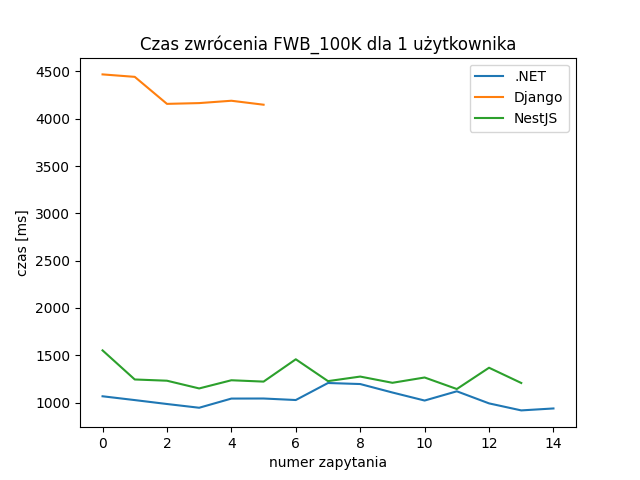
\includegraphics[width=1\linewidth]{rysunki/Czas_zwrocenia_FWB_100K_dla_1_uzytkownika.png}
	\caption{Czas zwrócenia zbioru FWB\_100K listy dla 1 użytkownika}
	\label{rys:request_duration_for_FWB_100K}
\end{figure}

Średni czas odpowiedzi na zapytanie zwracające zbiór FWB\_100K został zaprezentowany na rysunku \ref{rys:mean_duration_for_FWB_100K}.
Najdłuższy czas odpowiedzi uzyskał Django na poziomie 4,26 s.
Ponad 3 razy krótszy czas przypadł NestJS z wynikiem 1,27 s.
Najszybszym wynikiem wykazał się .NET z czasem 1,04 s. 

\begin{figure}[!hb]
	\centering 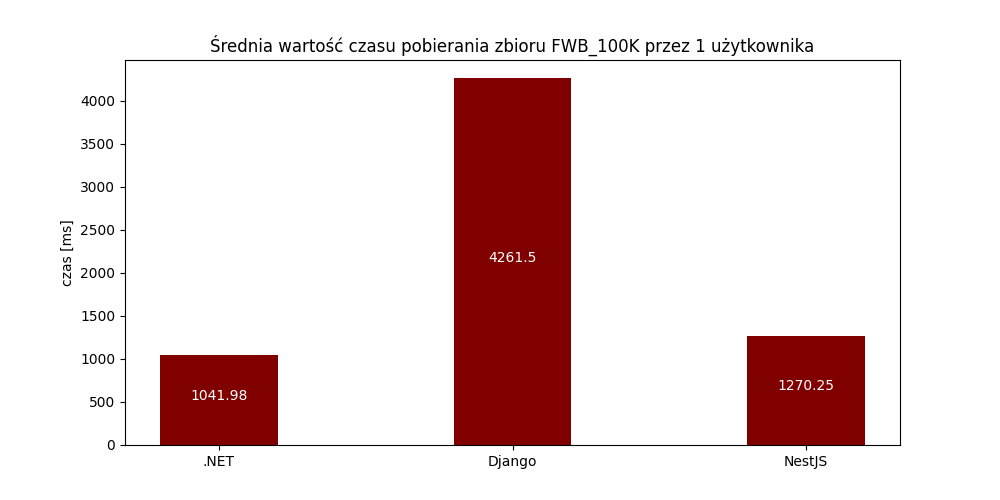
\includegraphics[width=1\linewidth]{rysunki/Srednia_wartosc_czasu_pobierania_zbioru_FWB_100K_przez_1_uzytkownika.png}
	\caption{Średni czas zwrócenia zbioru FWB\_100K dla 1 użytkownika}
	\label{rys:mean_duration_for_FWB_100K}
\end{figure}
